\chapter{Spint 0: Requirements gathering and Specification}

\phantomsection
\section*{Introduction}
\addcontentsline{toc}{section}{Introduction}
In this chapter, we place significant focus on gathering requirements and transforming them 
into well-defined and documented specifications. This includes creating use cases and user stories, 
which provide valuable insights into system interactions and user workflows. Furthermore, we establish 
a prioritized product backlog, ensuring efficient resource allocation and timely delivery of the most 
critical and valuable features. 

\section{Requirements gathering}
By conducting a comprehensive analysis of the requirements, we aim to bridge the gap between 
the stakeholders' vision and the actual implementation of the product or system. 
This analysis helps us define clear and concise specifications that serve as the foundation for the design, 
development, and testing phases of the project.

\subsection{Identifying end-users}
Identifying end-users is a crucial step in requirements analysis as it helps determine the needs, 
expectations, and constraints of the target audience. In our application, we were able to identify 
three types of actors:

\begin{itemize}
    \item \textbf{Administrator}: Is responsible for overseeing user accounts, configuring and maintaining the 
    resources needed by agents or employees to ensure the smooth operation of the system inside the organization.
    
    \item \textbf{Agent}: Is an employee inside the organization in charge of executing actions on the 
    notification center: creating and scheduling notification campaigns including the creation of
    notification content, client base segmentation. 

    \item \textbf{Client}: Is a customer who is going to be targeted by notifications from the business 
    or organization they belong to. A customer should be able to receive notifications and set their 
    preferences for receiving notifications from that business. 
\end{itemize}

\subsection{Functional requirements}
\label{freq}
Functional requirements define the specific actions, tasks, and behaviors that the product 
must be able to perform in order to meet the needs of its end-users. These requirements 
form the foundation of the system's functionality.

The functional requirements we captured for each actor in are outlined below.

\paragraph{Authentication and Profile settings}
\label{common-req}
\begin{itemize}
    \item \textbf{Sign in:} A registered user should be able to access the system by providing 
    valid credentials.
    \item \textbf{Edit profile settings:} A logged in user should be able to edit his profile settings.
    \item \textbf{View statistics:} A logged in user should be able to view notification activity metrics 
    on his dashboard.
\end{itemize}
\raggedbottom


\paragraph{Administrator requirements}
\label{admin-req}
\begin{itemize}
    \item \textbf{Manage agents:} An administrator should be able to add new agents, update,
    delete, desactivate accounts and reset passwords for existing agents.
    \item \textbf{Manage channels:} An administrator should be able to create new notification channels,
    update, delete, configure service providers for existing channels.
    \item \textbf{Manage topics:} An administrator should be able to create new notification topics,
    update, delete and configure topic's priority for existing ones.
\end{itemize}


\paragraph{Agent requirements}
\label{agent-req}
\begin{itemize}
    \item \textbf{Manage templates:} An agent should be able to create new notification templates, update and
    delete existing ones.
    \item \textbf{Manage triggers:} An agent should be able to create new notification triggers, configure
    the target audience the scheduling, update, change status and delete existing triggers.
    \item \textbf{Manage audiences:} An agent should be able create new segments of users based on a
    criteria, update and delete existing ones.
    \item \textbf{View logs:} An agent should be able to view logs of sent notifications and their statuses.
\end{itemize}

\paragraph{Client requirements}
\label{client-req}
\begin{itemize}
    \item \textbf{Manage notification preference:} A client should be able to edit his notification preferences,
    channels and frequency of receiving notifications.
    \item \textbf{View notification history:} A client should be able to checkout a history of his received 
    notifications (for in-app notifications).
\end{itemize}

\subsection{Non-Functional requirements}
\label{nfr}
When designing a notification system, various technical requirements need to be considered to ensure 
its effectiveness, reliability, and scalability. Here are the key requirements that should be addressed:

\begin{itemize}
    \item \textbf{Security:} The system shall enforce secure communication protocols, such as \acrshort{https}, 
    to protect sensitive data during transmissionn, also data and preferences stored in the system shall be securely 
    encrypted to prevent unauthorized access or data breaches.
    \item \textbf{Real-time:} The system shall deliver notifications in real-time or near real-time 
    to ensure timely communication, messages and notifications should be delivered with minimal delay for high 
    priority topics.
    \item \textbf{Scalability:} The system should be designed to handle a high volume of concurrent users 
    and notifications without compromising performance and the system architecture should be scalable, allowing for 
    horizontal scaling by adding more servers or utilizing cloud-based infrastructure as the user base grows.
    \item \textbf{Customizability:} The system should provide flexibility and customizability to meet 
    the specific branding and user experience requirements of different organizations. Also the system should 
    allow customization of user preferences to provide a personalized experience.
\end{itemize}

\section{Specification}
\label{spec}
In this section, we specify the system's requirements to lay the foundation for the development 
and implementation process and ensure that the final product meets the desired objectives.

\subsection{Global use case diagram}
Using \acrshort{uml} use case diagrams to model the requirements allows for a visual representation 
of the interactions between actors and the system, providing a clear and concise way to specify 
the functionalities and behaviors expected from the product.

The figure \ref{g-usecase} illustrates the global use case diagram we modeled for our notification system:

\begin{figure}[h!]
    \centering
    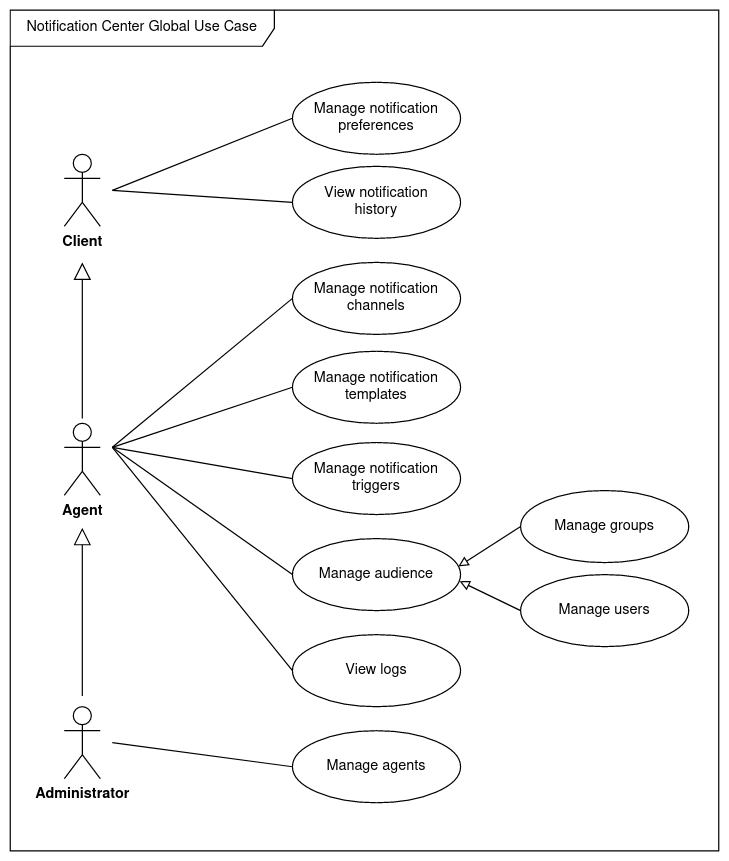
\includegraphics[width=\linewidth]{global-usecase.png}
    \caption{Notification Center global use case diagram}
    \label{g-usecase}
\end{figure}

\subsection{Product backlog}

\begin{longtable}{ | m{0.18\textwidth}  | m{0.49\textwidth} | c | c | }
        \hline
        \textbf{Epic} & \textbf{User story} & \textbf{Priority} & \textbf{Duration} \\
        \hline
        \endfirsthead
        \hline
        \textbf{Epic} & \textbf{User story} & \textbf{Priority} & \textbf{Duration} \\
        \hline  
        \endhead
        \hline
        \endfoot
        \endlastfoot
        \multirow{2}{5em}{Authentication} & As a new user, I want to be able to create an account so that I can use the notification center. & Must & 16 \\
        \cline{2-4}
        & As a registered user, I want to be able to log into my account securely using my email and password. & Must & 16 \\
        \hline
        \multirow{4}{5em}{Agents management} & As an administrator, I want to be able to create agents so that I can add them to the notification center. & Must & 16 \\
        \cline{2-4}
        & As an administrator, I want to be able to list agents so that I can view all registered agents. & Must & 16 \\
        \cline{2-4}
        & As an administrator, I want to be able to edit agents so that I can modify their information. & Must & 8 \\
        \cline{2-4}
        & As an administrator, I want to be able to delete agents so that I can get rid of no longer needed agents. & Must & 8 \\
        \hline
        \multirow{4}{5em}{Users management} & As an administrator/agent, I want to be able to create users so that I can send them notifications. & Must & 16 \\
        \cline{2-4}
        & As an administrator/agent, I want to be able to list users so that I can view all created users. & Must & 16 \\
        \cline{2-4}
        & As an administrator/agent, I want to be able to edit users so that I can modify their information. & Must & 8 \\
        \cline{2-4}
        &  As an administrator/agent, I want to be able to delete users so that I can get rid of no longer needed users. & Must & 8 \\
        \hline
        \multirow{4}{5em}{Audience management} & As an administrator/agent, I want to be able to create an audience so that I can target specific individuals based on a criteria. & Must & 24 \\
        \cline{2-4}
        & As an administrator/agent, I want to be able to list audiences so that I can view all created segments. & Must & 16 \\
        \cline{2-4}
        & As an administrator/agent, I want to be able to edit an audience so that I can change selection criteria and segment configurations. & Must & 8 \\
        \cline{2-4}
        & As an administrator/agent, I want to be able to delete a group of users so that I can get rid of no longer needed groups.. & Must & 8 \\
        \hline
        \multirow{4}{5em}{Notification channels management} & As an administrator/agent, I want to be able to create notification channels so that I can send notifications through these channels. & Must & 32 \\
        \cline{2-4}
        & As an administrator/agent, I want to be able to list notification channels so that I can view all created channels. & Must & 16 \\
        \cline{2-4}
        & As an administrator, I want to be able to edit notification channels so that I can modify or update their configurations. & Must & 8 \\
        \cline{2-4}
        & As an administrator/agent, I want to be able to delete notification channels so that I can get rid of no longer used channels. & Must & 8 \\
        \hline
        \multirow{4}{5em}{Notification templates management} & As an agent, I want to be able to add notification templates so that I can send notifications based on that template. & Must & 24 \\
        \cline{2-4}
        & As an agent, I want to be able to list notification templates so that I can view all created templates. & Must & 16 \\
        \cline{2-4}
        & As an agent, I want to be able to edit notification templates so that I can keep them up to date. & Must & 8 \\
        \cline{2-4}
        & As an agent, I want to be able to delete templates so that I can get rid of no longer used templates. & Must & 8 \\
        \hline
        Notification Preferences Management & As a user, I want to be able to set my notification preferences, so that I can receive notifications from the channels I want. & Must & 16 \\
        \hline
        \multirow{4}{5em}{Notification triggers management} & As an agent, I want to be able to create triggers for notifications so that I can schedule notifications to be sent automatically. & Must & 32 \\
        \cline{2-4}
        & As an agent, I want to be able to list triggers for notifications so that I can view all created triggers. & Must & 16 \\
        \cline{2-4}
        & As an agent, I want to be able to edit notifications triggers so that I can modify or update its configurations. & Must & 8 \\
        \cline{2-4}
        & As an agent, I want to be able to delete notification triggers so that I can get rid of outdated and no longer used triggers. & Must & 8 \\
        \hline
        \multirow{4}{5em}{Notification History} & As a user, I want to be able to list notification history so that I can review my received notifications whenever I want. & Must & 16 \\
        \cline{2-4}
        & As an administrator/agent, I want to be able to list sent notification logs so that I can review all sent notifications. & Must & 16 \\   
        \hline
        Dashboard & As an administrator/agent I want to be able to view metrics on my dashboard so that I can get an overview on important statistics related to notification activities. & Must & 16 \\
        \hline
        \caption{Backlog table}
\end{longtable}

\subsection{Sprints scheduling}

\phantomsection
\section*{Summary}
\addcontentsline{toc}{section}{Summary}
In this chapter, we translated requirements into specifications, encompassing the creation of use cases,
user stories, and a prioritized product backlog, ultimately setting the stage for subsequent phases 
of development.